
\section{Methodology}
\subsection{Image to Time-Series Encoding}
The nature of data in Stepscan dataset is a video-base dataset. There are several methods for converting a tensor (like video) to 2D time-series data. 

Chen et al. in \cite{Chen2006GaitModel} used contour width for defining a one-dimensional signal. They utilized some morphological operations on the background-subtracted silhouette image to extract the outer contour. Afterwards, according to the contour width of each image row, a one-dimensional signal was generated.

Another method could be that the pixel values in each frame are plotted over frame number. By this means, the $H * W$ time-series will be produced for each sample.

In the final method, some spatial features are extracted from each frame (e.g. centroid and maximum pressure in each frame). Afterwards, we track these values over time (next frames). As a result, 3D videos with size $T \times H \times W$ are converted to the four 2D time-series data. Costilla-Reyes et al. utilized this method to combine the output of 160 distributed \acrshort{pof} \cite{Costilla-Reyes2018DeepSensors}.

In this research, the last mentioned method was applied to produce time-series data. Figure \ref{fig:extracted_features} depicts the time series extracted from the Stepscan dataset. The spatial features extracted in each frame were maximum pressure (figure \ref{fig:extracted_features_max}), the center of pressure (COP) (figures \ref{fig:extracted_features_yCe} and \ref{fig:extracted_features_xCe}), and the average pressure (figure \ref{fig:extracted_features_sum}). 



\subsection{Conventional Classifiers}


The method consists of feature extraction, feature selection, and classification, as shown in Figure \ref{fig:flow}. In the following, each step would be described. 
 

\begin{center}
	\begin{figure*}[!t]
    	\centering
        \begin{minipage}[b]{\textwidth}
            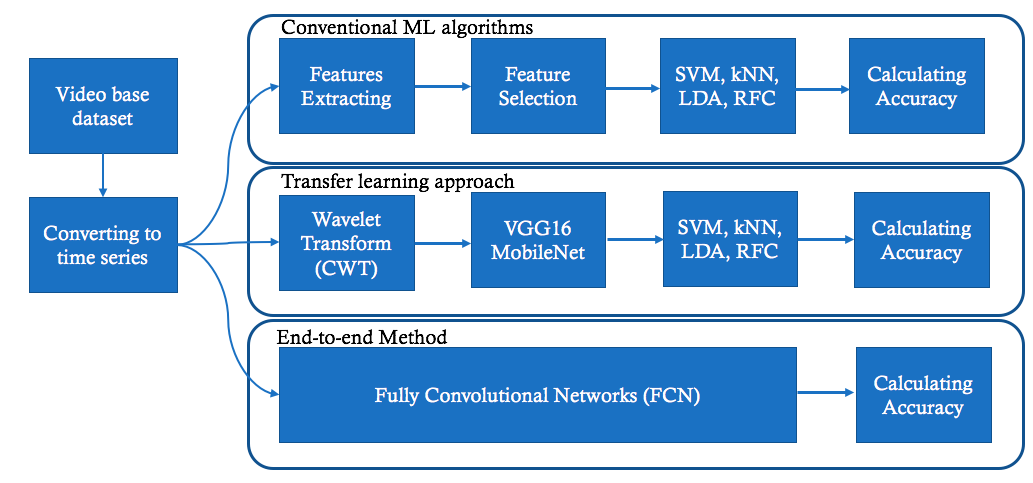
\includegraphics[width=\textwidth]{manuscript/src/figures/project/flowchart.png}
        \end{minipage}
        \hspace{-1em}
        \caption{Flowchart of implemented method.}
        \label{fig:flow}
	\end{figure*}
\end{center}

\subsubsection{Features Extraction and Selection}

As mentioned before, our goal is to develop a classification model. For this classification task, we use about $34$ features in four categories. These feature sets are explained briefly here, and more details about them can be found in Appendix A.

After extracting features from each time series, some low variance and high-correlated features were eliminated. Feature selection causes the complexity of the model to reduce. Ten percent of data were set aside for testing our classifier, and others were divided into 10-fold cross-validation for evaluation and training. 

To have equally balanced classes in the test set and cross-validation set, the methods Stratified and StratifiedKFold were used. Each set includes approximately the same percentage of samples of each class as the complete set. For example, if there are 10 samples out of 100 for class A, of stratified 3-fold cross-validation on a dataset with 50 samples from two unbalanced classes. We show the number of samples in each class and compare with KFold.%for extracting features from each time series, we need to consider a windows that size with over  Each group of features implemented on a size for extracting features from each time series, we need to consider a windows that  


\subsubsubsection{\textit{Temporal Features}.}
The first set of features extracted was temporal features. In this set, we focused on features that related to the time axis. Features like Entropy, Absolute energy, Centroid, Area under the curve fall into this group. The number of features extracted was 11.

\subsubsubsection{\textit{Statistical Features}.}
Statistical information was another feature set that was extracted from the dataset. Min, Max, variance, and standard deviation were some of the statistical features. The total number of features in this group is about 10 for each time series.  

\subsubsubsection{\textit{Spectral Features}.}
In the third category, both FFT and wavelet transform were used to extract spectral information from the dataset. Not only the time complexity but also the number of features were more than two other feature sets. 
Max power spectrum, Maximum frequency, Spectral centroid, Wavelet energy, and FFT mean coefficient were spectral features extracted from the dataset.

\subsubsubsection{\textit{\Gls{AR} coefficients}.}
The final set of features in this research was the coefficients of \gls{AR}. In this set, the first-order differencing used to make our data stationary. Then based on significant lag on \gls{PACF}, the order of the model  was selected. This approach extracted two features for each time-series signal.

\subsubsection{Machine learning algorithms}

These time-series features were fed to four different types of machine learning models with tuned hyper-parameters. The hyper-parameters tuning was implemented by grid search and performance evaluation with a 10  StratifiedKFold cross-validation. Table \ref{tab:1_ML} shows these models along with their best-tuned hyper-parameters.

\subsection{Deep Learning Approaches}
  
As Figure \ref{fig:flow} shows two approaches of Deep Neural Network were implemented. In this subsection, these approaches will be reviewed.


\subsubsection{Transfer Learning Approaches}
For this project, Two famous CNN architectures were implemented, including VGG16 \cite{Simonyan2015VeryRecognition}, and MobileNet \cite{Howard2017MobileNets:Applications}. These architectures complete feature extraction by automatically generating features from the raw footprint images. 
Due to the small size of the dataset, it is not possible to train networks on our dataset. As a result, pre-trained networks were downloaded from http://image-net.org/. The top layer of the CNN was eliminated and replaced with four machine learning algorithms like Random Forests, LDA, SVM, and kNN. 
A major limitation of the pre-trained networks is that the data is required to be of the type of image, while our data is time series. As a result the 2D-scalogram of each time-series signal were calculated and fed to CNNs. 


\subsubsection{Fully Convolutional Networks}
Another model which was implemented in this project is a Fully Convolutional Network (FCN) \cite{WangTimeBaseline}. This model is a end-to-end convolutional network with three blocks. Each block has a convolutional layer followed by a batch normalization and ReLU activation layer. The output of the third block is averaged over the time dimension which corresponds to global average pooling (GAP) layer. Finally, a softmax layer is fully connected to the GAP layer’s output to produce the final label.


